\documentclass[conference,letterpaper]{IEEEtran}
\usepackage{amsmath,amssymb,graphicx,booktabs,array,cite,url}
\usepackage[hidelinks]{hyperref}
\hypersetup{pdftitle={Evaluator Sensitivity of Client Contribution Scoring in Federated Wearable Learning},pdfauthor={Draft: authors pending confirmation}}
\newcommand{\TV}{\operatorname{TV}}
\newcommand{\CE}{\operatorname{CE}}
\newcommand{\R}{\mathbb{R}}
\newcommand{\E}{\mathcal{E}}
\title{Evaluator Sensitivity of Client Contribution Scoring in Federated Wearable Learning}
\author{\IEEEauthorblockN{Author information pending confirmation}}
\begin{document}
\maketitle
\begin{abstract}
Client contribution scores depend on the evaluation objective used to assign utility to a coalition. We study how this choice affects allocation while holding client updates fixed in a wearable activity-recognition setting. Using UCI HAR, we construct validation data exclusively from official training subjects, retain the official test split, and prespecify four cohorts of four clients. For each of ten independent training seeds, one-round client-update snapshots define all sixteen coalitions in each cohort. We compute exact Shapley values, leave-one-out scores, and data-size scores under sample-frequency, equal-class, and equal-subject evaluators. Allocation is defined by normalizing positive scores, with an explicit uniform fallback. Relative to sample-frequency evaluation, the mean within-seed, across-cohort total-variation distance between Shapley allocations is 0.12087 for equal-class evaluation and 0.00947 for equal-subject evaluation. Seed-level percentile bootstrap intervals at nominal 97.5\% are [0.10462, 0.13912] and [0.00801, 0.01100], respectively. The audit reconstructs 1,920 coalition utilities, 1,440 scores, and 240 ranking records and verifies 1,020 artifact hashes. The evidence supports a narrow conclusion: evaluator composition can materially change Shapley-based allocation in this fixed UCI HAR one-round setting. We make no claim of statistical significance, method superiority, general fairness, behavioral incentives, privacy guarantees, or generalization beyond this design.
\end{abstract}
\begin{IEEEkeywords}
federated learning, client contribution, Shapley value, evaluator sensitivity, human activity recognition, reproducibility
\end{IEEEkeywords}

\section{Introduction}
Federated learning separates local model fitting from model aggregation. The model-averaging approach introduced by McMahan et al.~\cite{fedavg} provides a familiar basis for studying clients whose datasets differ in size and composition. A separate question concerns attribution: given a collection of client updates, how should their contributions to an evaluation objective be described? This question arises even when the training algorithm, client participation, and model checkpoint are already fixed. Contribution evaluation is therefore a distinct experimental object, not simply another name for model accuracy.

A coalition receives value only after an evaluator is specified. In activity recognition, an evaluator can average losses over all available windows, first average within each activity and then across activities, or first average within each person and then across people. These choices use the same model predictions and labels but give different importance to individual observations. A client update that helps one part of the evaluation set can consequently receive different credit under different evaluators. This dependence is mathematically expected. Its magnitude in an explicitly controlled wearable-learning experiment is the empirical question addressed here.

Shapley values offer a principled description of marginal contributions within a specified cooperative game~\cite{shapley}. Their exact computation does not remove choices about that game's utility, coalition construction, or downstream score normalization. In particular, computing all coalitions can remove coalition-sampling approximation while leaving evaluator dependence intact. It is important to distinguish exactness with respect to the chosen game from a claim that the game yields a unique or universally appropriate value for a client.

This paper studies that distinction using a deliberately bounded design. We use the public UCI HAR smartphone activity-recognition dataset~\cite{har,uci}, sixteen subject-clients, four fixed cohorts, and ten independent training seeds. Every cohort has four clients, permitting exhaustive evaluation of its sixteen coalitions. All client snapshots within a seed start from the same final warmup model. The snapshots and resulting coalition predictions are reused under all evaluators. Thus, evaluator comparisons do not retrain a model, resample a coalition, or change the local update budget.

The primary question is: \emph{with client updates, coalition aggregation, validation observations, and scoring rule held fixed, how much does changing evaluator composition alter normalized Shapley allocation?} Here, evaluator composition means the empirical weighting of the existing validation observations; it does not mean changing which observations are present. The two prespecified contrasts compare equal-class and equal-subject evaluation with sample-frequency evaluation. We use leave-one-out and data-size scoring as secondary references, without treating either as ground truth for exact Shapley values.

Our contribution is a controlled empirical characterization with a reproducible audit trail. First, we define the complete one-round game, three evaluation measures, and the transformation from signed scores to allocations. Second, we separate evaluator choice from update generation using exhaustive four-client coalition evaluation. Third, we report all ten seed-level primary observations and uncertainty estimates, supported by independent numerical reconstruction and pre-completion integrity checks. We do not propose a new valuation algorithm, scheduling rule, or incentive mechanism.

\section{Related Work and Scope}
\subsection{Valuation and the choice of a game}
Shapley's foundational value assigns credit using marginal changes across coalitions~\cite{shapley}. Data Shapley adapts this idea to the value of training observations for a learning task and develops computational approximations~\cite{datashapley}. Our players are subject-client updates, rather than individual training windows. We keep the model-update snapshots fixed and evaluate their aggregate models. Consequently, our exact values belong to an update-combination game, not a game in which each coalition trains a new predictor from its pooled raw data.

Distributional Shapley explicitly places data valuation in the context of an underlying distribution~\cite{distributional}. This is relevant background for recognizing that valuation is conditional on its statistical setting. We do not estimate distributional Shapley values or adopt its guarantees. Our evaluator distributions are three finite weighting schemes over one fixed held-out validation set. The distinction matters: variation across training seeds in this study does not represent sampling uncertainty over validation subjects or over a broader wearable population.

\subsection{Contribution evaluation in federated learning}
GTG-Shapley reconstructs federated models from updates and uses guided sampling and truncation to reduce contribution-evaluation cost~\cite{gtg}. Reusing updates is therefore established practice, and we do not claim this reconstruction principle as new. Our four-client setting permits complete coalition enumeration, so guided sampling and truncation are unnecessary. This design removes one computational approximation from the evaluator comparison; it does not demonstrate that exact enumeration is preferable at larger scale.

Chen et al.~\cite{flce} provide a comprehensive experimental evaluation of federated contribution estimation and distinguish utility metrics, estimation schemes, and computational optimizations. Their work is a direct precedent for empirical studies in this area. Our study is narrower: the coalition models are fixed while three validation weighting schemes are crossed with three scoring references. We do not claim to replace a broad benchmark or to comprehensively evaluate the effectiveness, robustness, or efficiency of contribution methods.

ShapFed considers class-specific contributions and uses contribution information in aggregation and personalization~\cite{shapfed}. It already motivates moving beyond a single undifferentiated performance summary. We neither implement ShapFed nor compare prediction performance against it. Our equal-class evaluator is a fixed reweighting of validation cross-entropy, without class-specific personalized models or an adaptive aggregation loop.

The closest conceptual overlap is Maverick-aware Shapley valuation, which reweights validation scores using per-class performance and connects the resulting values to client selection~\cite{rare}. That work makes a broad claim that evaluator-sensitive valuation is new untenable. Our distinction is an auditable fixed-update sensitivity study using three prespecified empirical measures, exact small-coalition calculations, and seed-level allocation distances. We make no claim that this distinction establishes algorithmic novelty. The institutional abstract and bibliographic record for~\cite{rare} were verified; detailed full-text comparisons remain flagged for manual confirmation in the submission companion.

\begin{table}[t]
\caption{Position relative to verified prior work. These are scope distinctions, not performance comparisons.}
\label{tab:related}\centering\small
\begin{tabular}{p{.25\columnwidth}p{.63\columnwidth}}\toprule
Prior work & Relationship to this study\\\midrule
Data Shapley~\cite{datashapley} & Established valuation framework; our players are fixed client updates.\\
GTG-Shapley~\cite{gtg} & Established update reconstruction; we enumerate all small-cohort coalitions.\\
FLCE evaluation~\cite{flce} & Broad evaluation precedent; our intervention is validation weighting.\\
ShapFed~\cite{shapfed} & Class-aware contribution precedent; no personalization or adaptive aggregation here.\\
Maverick-aware valuation~\cite{rare} & Validation reweighting precedent; no performance-adaptive evaluator or client-selection feedback here.\\\bottomrule
\end{tabular}
\end{table}

\subsection{Wearable-learning context}
UCI HAR provides subject identifiers and a fixed activity-recognition dataset~\cite{har,uci}. These enable natural subject-clients and a subject-disjoint validation construction. We use the wearable setting to make the evaluation unit meaningful: a window, an activity class, and a person are different ways to summarize the same predictions. This is not an on-device deployment study. The experiments run in a local process and do not measure network behavior, wearable energy, real-world availability, or clinical outcomes. Table~\ref{tab:related} summarizes the scope of the literature comparison.

\section{Fixed-Update Contribution Game}
\subsection{Clients, cohorts, and snapshots}
Let $s\in\{4101,\ldots,4110\}$ denote a training seed and let $c\in\{A,B,C,D\}$ denote a prespecified cohort. Each cohort has a set $N_c$ of four clients. Client $i$ has $n_i$ training windows. For clarity, we suppress $s$ and $c$ in equations when they are not needed. The final warmup model for a seed is $\theta_0$. Client $i$ performs its fixed local work starting at $\theta_0$, producing $\theta_i$ and update
\begin{equation}
\Delta_i=\theta_i-\theta_0.
\end{equation}
The same $\Delta_i$ is used in every coalition that contains $i$. No coalition-specific local training is performed.

For $S\subseteq N_c$, the coalition model is
\begin{equation}
\theta_S=\begin{cases}
\theta_0,&S=\varnothing,\\
\displaystyle\theta_0+\sum_{i\in S}\frac{n_i}{\sum_{k\in S}n_k}\Delta_i,&S\ne\varnothing.
\end{cases}
\label{eq:coalition}
\end{equation}
All sixteen subsets are included. Client order is ascending subject identifier; a four-bit coalition mask uses this fixed order. The empty coalition retains the base model, and a singleton contains that client's update without dilution by absent clients. The aggregation denominator depends on the coalition, so a client's marginal contribution includes the effect of renormalizing the participating update weights.

The base model was trained using all sixteen training clients before cohorts were evaluated. The contribution game therefore concerns \emph{an additional update from an already represented client}. It does not measure the value of introducing that client's data into a model that has never seen it. Moreover, cohort $N_c$ is the grand coalition only for its own four-player game, not for the entire sixteen-client federation. These boundaries are essential to interpreting the scores.

\subsection{Three evaluators on identical observations}
Let the validation set be $V=\{(x_j,y_j,u_j)\}_{j=1}^{M}$, where $u_j$ is a validation subject identifier and $y_j\in\{0,\ldots,5\}$ is an activity label. In this study $M=1783$ and five subjects are represented. Define $M_k=|\{j:y_j=k\}|$ and $M_u=|\{j:u_j=u\}|$. All six classes occur in validation. For evaluator $e$, weighted cross-entropy is
\begin{equation}
L_e(\theta)=\sum_{j=1}^{M}w_j^{(e)}\ell(\theta;x_j,y_j),\qquad
\ell=-\log p_\theta(y_j\mid x_j).
\label{eq:loss}
\end{equation}
Weights are nonnegative and sum to one. The three definitions are
\begin{align}
w_j^{(F)}&=\frac{1}{M},\label{eq:f}\\
w_j^{(C)}&=\frac{1}{6M_{y_j}},\label{eq:c}\\
w_j^{(U)}&=\frac{1}{5M_{u_j}}.\label{eq:u}
\end{align}
$F$ is sample-frequency evaluation: each window receives equal weight. $C$ gives each class total weight $1/6$, with equal window weights within class. $U$ gives each validation subject total weight $1/5$, with equal window weights within subject. Equal-subject evaluation does not give equal weight to training clients; its groups are the five distinct validation subjects. Neither $C$ nor $U$ is an inverse-propensity estimator for an unknown population.

The utility of a coalition is the reduction in weighted validation loss relative to the fixed base:
\begin{equation}
v_e(S)=L_e(\theta_0)-L_e(\theta_S).
\label{eq:utility}
\end{equation}
Thus $v_e(\varnothing)=0$. Positive utility indicates lower cross-entropy under evaluator $e$; negative utility is allowed. Evaluation uses saved float32 model logits, with losses and utility calculations performed in float64. The three evaluators reuse exactly the same predictions. Their differences are solely consequences of the fixed weighting definitions in (\ref{eq:f})--(\ref{eq:u}).

\subsection{Exact Shapley and scoring references}
For four players, the exact Shapley score is
\begin{equation}
\phi_i^{(e)}=\sum_{S\subseteq N_c\setminus\{i\}}
\frac{|S|!(3-|S|)!}{4!}
\big[v_e(S\cup\{i\})-v_e(S)\big].
\label{eq:shapley}
\end{equation}
Every term is available because all sixteen utilities have been computed. Exactness here means complete finite-coalition enumeration up to floating-point arithmetic. It does not refer to exact learning optimization or exact population utility. The audit independently averages marginal contributions over all $4!=24$ player permutations and checks the efficiency identity
\begin{equation}
\sum_{i\in N_c}\phi_i^{(e)}=v_e(N_c)-v_e(\varnothing).
\label{eq:efficiency}
\end{equation}

Two additional scoring references use the same cohort:
\begin{align}
q_i^{(e)}&=v_e(N_c)-v_e(N_c\setminus\{i\}),\label{eq:loo}\\
d_i&=\frac{n_i}{\sum_{k\in N_c}n_k}.\label{eq:size}
\end{align}
Equation~(\ref{eq:loo}) is leave-one-out (LOO), the marginal contribution at the grand coalition. It is a distinct rule, not an unbiased approximation to (\ref{eq:shapley}). Equation~(\ref{eq:size}) is data-size scoring. It is intentionally independent of evaluator weights and serves as a negative control for the evaluator-comparison pipeline. Its invariance does not make it an adequate measure of utility contribution.

\subsection{From signed scores to allocation shares}
Shapley and LOO scores may be negative. We retain signed scores in the raw evidence and define a separate allocation transformation. For a score vector $a=(a_i)_{i\in N_c}$, write $a_i^+=\max(a_i,0)$. The share vector is
\begin{equation}
r_i(a)=\begin{cases}
\displaystyle a_i^+/\sum_{k\in N_c}a_k^+,&\sum_k a_k^+>0,\\
1/4,&\sum_k a_k^+=0.
\end{cases}
\label{eq:allocation}
\end{equation}
The uniform fallback is explicitly flagged. This transformation is an experimental convention, not an incentive mechanism. The efficiency identity applies to signed Shapley scores, not to these normalized shares. Clipping and normalization can change the geometry of score differences, which is why signed-score and fallback diagnostics are reported separately.

\subsection{Total variation and its interpretation}
For two allocation vectors $r,r'\in\R^4$ with nonnegative entries summing to one, total variation is
\begin{equation}
\TV(r,r')=\frac{1}{2}\sum_{i\in N_c}|r_i-r_i'|.
\label{eq:tv}
\end{equation}
It lies in $[0,1]$ and equals the sum of positive share changes, the magnitude of the sum of negative share changes, and the maximum allocation-mass difference over client subsets. It can be interpreted as the fraction of a unit allocation that must be reassigned to transform one share vector into the other. Zero means identical allocations; one means disjoint positive support. The factor $1/2$ avoids counting the same transferred mass at both its origin and destination.

The primary cohort-level contrasts use $r(\phi^{(C)})$ versus $r(\phi^{(F)})$ and $r(\phi^{(U)})$ versus $r(\phi^{(F)})$. We do not compute TV directly between signed Shapley vectors, which need not be probability vectors. Nor is allocation TV a distance between label distributions or a change in accuracy. A cohort TV of 0.12 means a 12\% redistribution of normalized unit mass in that cohort, not a 12-percentage-point change for every client.

\section{Data and Update-Generation Protocol}
\subsection{Official split and validation construction}
UCI HAR contains smartphone inertial recordings from thirty people performing six activities~\cite{har,uci}. We retain the publisher's 128-sample windows and preprocessing. The original windows have 50\% overlap. Model inputs are the nine supplied channels: three axes each of body acceleration, body gyroscope, and total acceleration. We do not use the engineered 561-feature representation or generate additional windows.

The official training set has 7,352 windows from twenty-one subjects; the official test set has 2,947 windows from nine other subjects. Validation is constructed exclusively from official training subjects. Sorting their identifiers, we select positions 1, 5, 9, 13, and 17 (one-based): subjects 1, 7, 15, 21, and 26. Their 1,783 windows form validation. The remaining sixteen subjects supply 5,569 training windows. Every official training window belongs exactly once either to one training client or to validation.

The fixed clients are grouped as shown in Table~\ref{tab:cohorts}. Cohorts are not optimized for label balance, contribution magnitude, or evaluator sensitivity. All cohorts are retained in every seed. The subject holdout avoids splitting neighboring overlapping windows of the same person between training and validation. Additional checks find no identical windows across training, validation, and official test splits. This does not establish independence among windows within a subject, and no analysis treats them as independent experimental replications.

\begin{table}[t]
\caption{Fixed subject cohorts and training-window counts, in ascending subject order. Validation subjects are 1, 7, 15, 21, and 26.}
\label{tab:cohorts}\centering\small
\begin{tabular}{cll}\toprule
Cohort & Subject identifiers & Respective window counts\\\midrule
A & 3, 5, 6, 8 & 341, 302, 325, 281\\
B & 11, 14, 16, 17 & 316, 323, 366, 368\\
C & 19, 22, 23, 25 & 360, 321, 372, 409\\
D & 27, 28, 29, 30 & 376, 382, 344, 383\\\bottomrule
\end{tabular}
\end{table}

Each channel is standardized using its mean and standard deviation fitted across the windows and time positions of the sixteen training clients only. Validation and test data use these fixed statistics. Neither validation nor test statistics enter normalization. The official class order is walking, walking upstairs, walking downstairs, sitting, standing, and laying, mapped to integers 0--5. The label mapping, split membership, and normalization arrays are saved.

\subsection{Model and warmup}
The classifier has two one-dimensional convolutional layers: nine to sixteen channels and sixteen to thirty-two channels, each with kernel size five, padding two, and ReLU activation. Temporal mean pooling and maximum pooling are concatenated to form a 64-dimensional representation. A linear layer produces six logits. There is no batch normalization or dropout. The model is intentionally compact; no claim is made that it is an optimal HAR architecture.

For each seed, twenty full-participation FedAvg warmup rounds train a shared base model. All sixteen clients participate in every warmup round. Each local invocation starts from the current global parameters and performs \emph{five local minibatch steps}, with batch size 64 and stochastic gradient descent at learning rate 0.03, zero momentum, and zero weight decay. A fresh optimizer is created for each invocation. Client windows are visited in a shuffled permutation; a short final minibatch is retained, and a new permutation is drawn only when the previous one is exhausted. Local work is specified in steps, not epochs.

Warmup aggregation uses client training-window counts. The final round-twenty model is the base $\theta_0$ regardless of its validation or test performance. There is no checkpoint search, early stopping, or evaluator-dependent training. In particular, the equal-class and equal-subject definitions are valuation objectives only. They do not reweight the local training loss.

\subsection{One-round snapshots and common randomness}
Each of the sixteen clients then performs five additional minibatch steps from the same $\theta_0$. Its resulting update is saved once and used for all relevant coalitions. Although twenty warmup rounds precede this stage, the contribution game itself is one round: it attributes these fixed additional updates. No sequence of coalition-specific federated trajectories is evaluated.

Seeds 4101--4110 are fixed in advance. Separate pseudorandom streams are derived with SHA-256 from the seed and invocation identifiers for initialization, warmup round/client, and snapshot client. Evaluator comparisons within a seed share the base model, updates, coalitions, validation observations, and data counts. Across seeds, the split, cohorts, architecture, and hyperparameters remain fixed, while initialization and minibatch permutations vary. Thus, seeds represent repeated training randomness conditional on one data design.

All runs use deterministic PyTorch operations on CPU with one thread. The recorded environment includes Python 3.12.14, PyTorch 2.14.0+cpu, and NumPy 2.3.5. This is a local federated-learning simulation; it does not require a distributed execution framework or claim real-device timing. Table~\ref{tab:protocol} collects the settings needed to reconstruct the experiment.

\begin{table}[t]
\caption{Frozen protocol. No setting was selected using official test performance.}
\label{tab:protocol}\centering\small
\begin{tabular}{p{.40\columnwidth}p{.50\columnwidth}}\toprule
Item & Fixed setting\\\midrule
Training / validation / test windows & 5,569 / 1,783 / 2,947\\
Training clients / cohorts & 16 subjects / 4 fixed groups\\
Players per game / coalitions & 4 / all 16 subsets\\
Warmup & 20 rounds; all 16 clients\\
Local work & 5 minibatch steps per invocation\\
Optimizer & SGD; learning rate 0.03\\
Momentum / weight decay & 0 / 0\\
Batch size & 64; retain short final batch\\
Model & Conv1D 9--16--32; mean/max pooling; linear 64--6\\
Contribution stage & One snapshot update per client\\
Seeds & 4101--4110\\
Primary uncertainty & 50,000 seed bootstrap resamples\\
Bootstrap RNG seed & 91001\\\bottomrule
\end{tabular}
\end{table}

\subsection{Test-set separation}
All coalition logits, utilities, scores, shares, and ranking comparisons are persisted and hashed before a valuation-freeze record is written. Only then does the experimental runner load the official test split. It evaluates the base and the four full-cohort models descriptively. The official test labels do not enter client construction, coalition weighting, contribution scoring, checkpoint choice, hyperparameter selection, or stopping. Data-integrity tests can inspect split identifiers and duplicate content, but test performance is not used in experimental decisions.

\section{Measures, Uncertainty, and Integrity}
\subsection{Seed-level estimands}
For each seed and evaluator contrast $e\in\{C,U\}$, define
\begin{equation}
D_{s,c}^{(e)}=\TV\big(r(\phi_{s,c}^{(e)}),r(\phi_{s,c}^{(F)})\big)
\end{equation}
and the within-seed cohort mean
\begin{equation}
\bar D_s^{(e)}=\frac{1}{4}\sum_{c\in\{A,B,C,D\}}D_{s,c}^{(e)}.
\label{eq:seedmean}
\end{equation}
The reported mean is $10^{-1}\sum_s\bar D_s^{(e)}$; the median is taken over the same ten values. TV is computed before averaging across cohorts. Pooling client shares from distinct games first would define a different quantity, because each cohort has its own unit allocation and normalization denominator.

The independent unit is the training seed. Four cohorts within a seed share a base model and are fixed repeated blocks. Three evaluators reuse identical predictions. Sixteen coalitions reuse the same updates. None of these are additional independent experimental units. The 1,920 utility records improve traceability and permit exact reconstruction, but do not turn this experiment into a study with 1,920 independent replicates.

\subsection{Bootstrap intervals}
We use a nonparametric seed bootstrap, following the resampling principle introduced by Efron~\cite{efron}. For each of 50,000 resamples, ten seed indices are drawn with replacement from the observed ten seeds. The same index matrix is applied to both primary contrasts. Each resample yields a mean of ten within-seed cohort means. The 0.0125 and 0.9875 empirical quantiles form a nominal 97.5\% percentile interval for each contrast.

The per-contrast level is chosen for the two prespecified primary means, targeting approximately 95\% family coverage using a Bonferroni adjustment. This target depends on the quality of each bootstrap interval; ten seeds do not provide an exact finite-sample coverage guarantee. Median intervals at the same nominal level are retained as descriptive outputs, not an expanded confirmatory family. No hypothesis tests or $p$-values are computed, and interval endpoints are not interpreted as establishing statistical significance.

Resampling seeds holds the observed subjects, cohorts, preprocessing, model, and update budget fixed. These intervals quantify uncertainty associated with repeated training randomness under that conditional design. They do not incorporate alternative subject samples, validation constructions, cohort assignments, or datasets. A narrow interval in this analysis cannot compensate for the absence of those forms of replication.

\subsection{Secondary descriptive measures}
For signed scores, each cohort has six unordered client pairs. A strict rank reversal occurs when the sign of a pairwise score difference changes between evaluators. Differences within $10^{-8}$ are treated as ties. Ties and tie transitions are recorded rather than broken to create a strict ranking. The outputs also include tolerance-aware Kendall's $\tau_b$ and overlap of top-ranked sets; $\tau_b$ is recorded as undefined when its denominator is zero.

LOO and data-size allocations are compared with Shapley allocations using the same TV definition. These disagreements describe differences between scoring rules; they are not estimation errors against an externally verified notion of client value. Negative-score fractions and uniform-fallback frequencies disclose how the allocation transformation interacts with the signed scores. Secondary figures are exploratory descriptive summaries and are not assigned significance claims.

\subsection{Completion gate and independent reconstruction}
A run writes artifacts through temporary files, flushes and fsyncs them, atomically replaces final paths, and fsyncs containing directories where supported. Files are closed before the artifact manifest is generated. A separate audit process verifies the required inventory, hashes, counts, coalition masks, evaluator utilities, scores, rankings, and leakage controls. It reconstructs coalition parameters from saved updates and recomputes predictions. It independently evaluates Shapley values through all twenty-four permutations rather than reusing the subset implementation.

The audit also reconstructs weighted losses from saved validation logits and labels, checks the Shapley efficiency residual against $10^{-12}$, and reproduces allocation and ranking calculations. Only after all checks pass does the runner create \texttt{COMPLETE.json}, which records the manifest and audit hashes. Post-completion audits verify the marker and ordering again. Regression tests inject an incorrect ranking, a missing file, an extra file, and a missing manifest entry; each prevents completion marking. The full unit and regression suite passed 26 tests before the corrected pilot.

All ten accepted runs use the frozen \texttt{study-v1.1} release. The corrected seed-4101 pilot is counted once; its earlier validation copy is excluded from the ten-seed sample. Seeds 4102--4110 each ran once. No failed or incomplete run entered analysis, and no seed was retried, replaced, or selected by its outcome. After all runs, a new cross-seed audit checked common splits, normalization, environment, configuration, source version, and distinct initializations before descriptive analysis began.

\section{Audited Results}
\subsection{Evidence completeness}
Table~\ref{tab:audit} reports the accepted evidence. Ten seeds, four cohorts, sixteen coalitions, and three evaluators yield $10\times4\times16\times3=1920$ utility records. Three scoring references and four clients yield $10\times4\times3\times3\times4=1440$ score records. The 240 ranking records are $10\times4\times3\times2$, one for each seed, cohort, scoring reference, and contrast against sample-frequency evaluation. These counts are planned inventory requirements, not independent sample sizes.

All 1,020 raw artifact-manifest entries verified. The twelve Shapley games per seed passed the efficiency check; the largest residual across 120 games was $1.39\times10^{-17}$. The audit reconstructed 640 coalition-model entries and 150 descriptive test metrics. Common split, normalization, validation-index, and environment hashes matched across seeds. Each seed had a distinct initial-model hash. These checks support faithful execution of the specified experiment, while not proving that every scientific assumption or shared code component is correct.

\begin{table}[t]
\caption{Complete ten-seed integrity audit. Record counts are not statistical sample sizes.}
\label{tab:audit}\centering\small
\begin{tabular}{lr}\toprule
Audited object & Passed / expected\\\midrule
Independent seeds & 10 / 10\\
Coalition-model entries & 640 / 640\\
Evaluator utilities & 1,920 / 1,920\\
Client contribution scores & 1,440 / 1,440\\
Ranking-comparison records & 240 / 240\\
Raw artifact hashes & 1,020 / 1,020\\
Shapley efficiency checks & 120 / 120\\
Descriptive test-metric checks & 150 / 150\\\midrule
Maximum efficiency residual & $1.39\times10^{-17}$\\\bottomrule
\end{tabular}
\end{table}

\subsection{Primary evaluator contrasts}
Table~\ref{tab:primary} and Fig.~\ref{fig:primary} present the primary measurements. Equal-class versus sample-frequency evaluation has mean Shapley-allocation TV 0.120866, median 0.114539, and nominal 97.5\% mean interval [0.104623, 0.139118]. Equal-subject versus sample-frequency evaluation has mean 0.009466, median 0.009475, and interval [0.008006, 0.010998]. The table reports additional digits for reproducibility; these should not be interpreted as corresponding practical precision.

The first mean corresponds to approximately 12.09\% of a normalized unit allocation being reassigned, averaged over cohorts within seeds and then over seeds. The second corresponds to approximately 0.95\%. The contrast between these two magnitudes is descriptive within the fixed design; we have not tested whether the contrasts differ statistically. Neither magnitude is an accuracy improvement, a welfare gain, or evidence that one evaluator should be adopted.

We use ``materially change'' in the narrow descriptive sense that the equal-class contrast reallocates a nontrivial fraction of the unit allocation in this experiment. No external practical-importance threshold, monetary scale, or clinical consequence was prespecified or measured. The numerical distances, rather than that adjective, are the primary evidence. The observed change cannot be attributed to different client training runs across evaluators, because all evaluator variants reuse the same coalition logits.

\begin{table*}[t]
\caption{Primary seed-level Shapley-allocation TV summaries. Means and medians are over ten independent seeds after averaging four fixed cohorts within each seed. Intervals are percentile seed-bootstrap intervals, not significance tests.}
\label{tab:primary}\centering
\begin{tabular}{lrrrr}\toprule
Contrast against sample-frequency & Mean TV & Median TV & Seed SD & 97.5\% interval for mean\\\midrule
Equal-class & 0.120866 & 0.114539 & 0.025598 & [0.104623, 0.139118]\\
Equal-subject & 0.009466 & 0.009475 & 0.002239 & [0.008006, 0.010998]\\\bottomrule
\end{tabular}
\end{table*}

\begin{figure*}[t]
\centering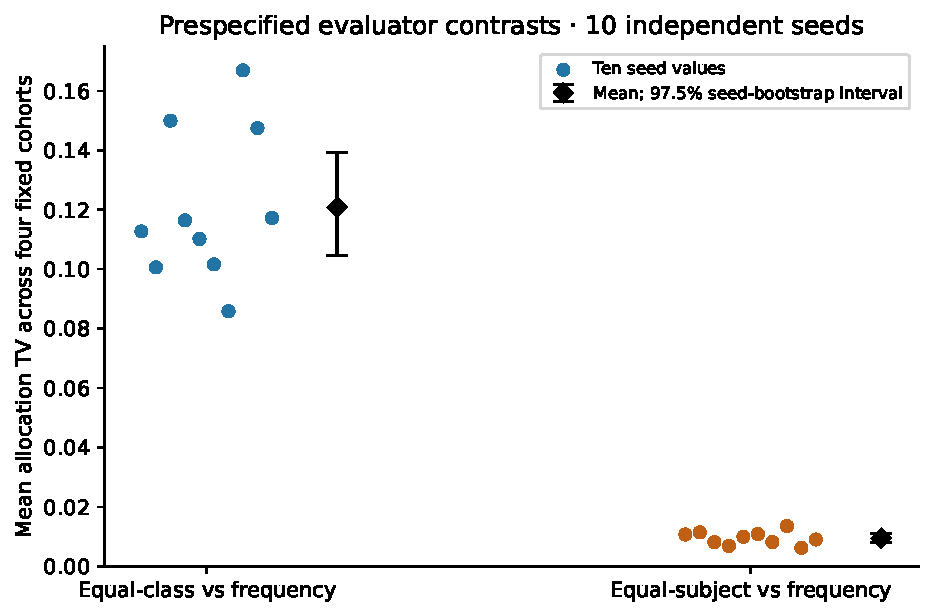
\includegraphics[width=.76\textwidth]{figures/primary_seed_intervals.pdf}
\caption{Primary evaluator contrasts. Each point is one seed's mean over four fixed cohorts; horizontal offsets distinguish points and have no statistical meaning. Black diamonds denote means, with nominal 97.5\% percentile bootstrap intervals based on resampling the ten seeds. No subjects, windows, or coalitions are resampled.}
\label{fig:primary}
\end{figure*}

\subsection{All prespecified seeds}
Table~\ref{tab:seeds} reports every seed. The equal-class values range from 0.085805 to 0.166881; equal-subject values range from 0.006176 to 0.013511. We include the full list to make the relationship between the plotted observations and summary statistics inspectable. No favorable seed or illustrative cohort was selected for the primary presentation.

\begin{table}[t]
\caption{All primary within-seed cohort means. Each row is one independent unit.}
\label{tab:seeds}\centering\small
\begin{tabular}{rrr}\toprule
Seed & Equal-class vs frequency & Equal-subject vs frequency\\\midrule
4101 & 0.112687 & 0.010687\\
4102 & 0.100605 & 0.011415\\
4103 & 0.149963 & 0.008116\\
4104 & 0.116391 & 0.006856\\
4105 & 0.110145 & 0.009945\\
4106 & 0.101584 & 0.010809\\
4107 & 0.085805 & 0.008142\\
4108 & 0.166881 & 0.013511\\
4109 & 0.147437 & 0.006176\\
4110 & 0.117159 & 0.009005\\\bottomrule
\end{tabular}
\end{table}

\subsection{Rank changes and scoring-reference diagnostics}
Figure~\ref{fig:ranks} shows the descriptive rank-reversal fractions for all four cohorts and all three scoring references. Each cell averages, over ten seeds, the fraction of the six client pairs that strictly reverse. This representation retains cohort structure without assigning forty independent observations to a contrast. The data-size row is zero, as required by its evaluator-independent definition. This negative control would reveal an error if evaluator changes altered data-size ranks or shares.

Figure~\ref{fig:references} shows allocation disagreement between LOO or data-size scoring and exact Shapley, with each point again representing a within-seed cohort mean. The comparisons do not identify the ``best'' scorer. Exact Shapley is the reference for a stated cooperative game; LOO asks a different marginal question, and data-size ignores utility. Numerical agreement or disagreement among them alone cannot establish correctness with respect to an external allocation objective.

\begin{figure*}[t]
\centering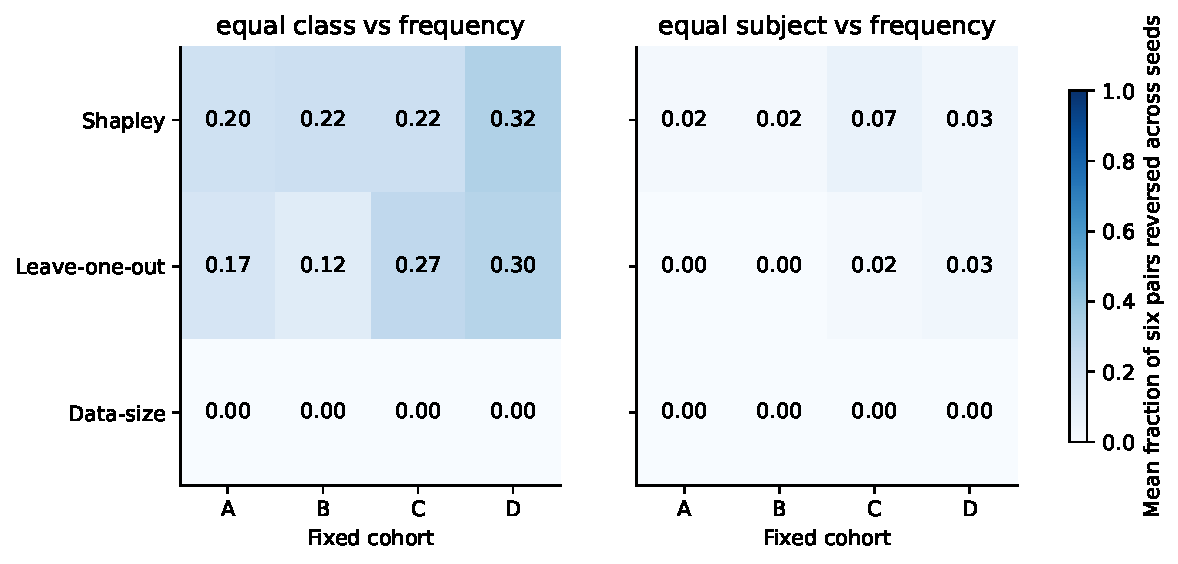
\includegraphics[width=.84\textwidth]{figures/rank_reversal_descriptive.pdf}
\caption{Exploratory rank diagnostics across all fixed cohorts. Cells are mean fractions of six unordered client pairs whose signed-score ordering strictly reverses across the indicated evaluator contrast. Ties use tolerance $10^{-8}$. The heatmap is descriptive and has no inferential interpretation at the client-pair level.}
\label{fig:ranks}
\end{figure*}

\begin{figure*}[t]
\centering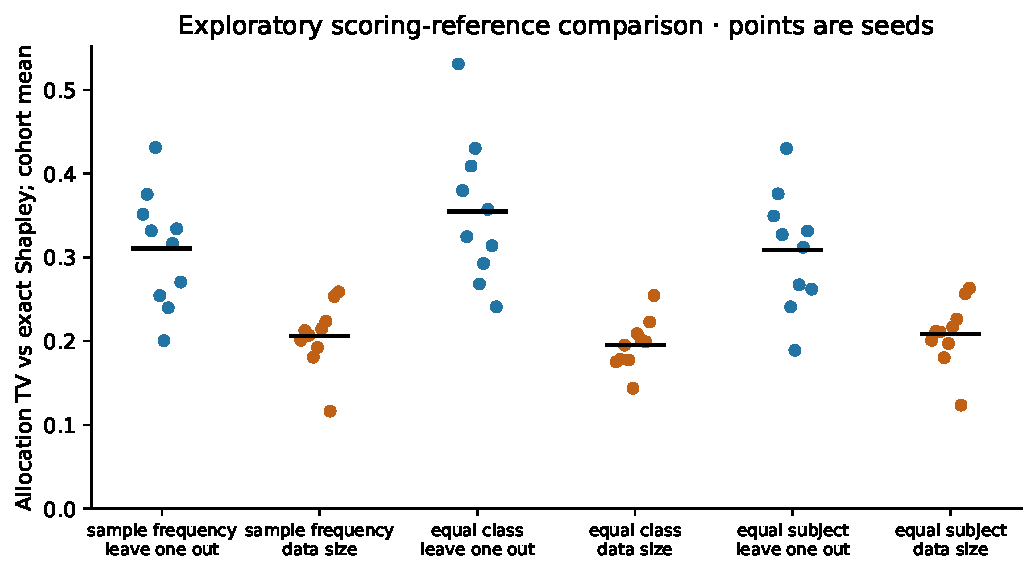
\includegraphics[width=.84\textwidth]{figures/scoring_reference_disagreement.pdf}
\caption{Exploratory allocation disagreement with exact Shapley under each evaluator. Points are ten seed-level means over four cohorts; horizontal black marks are means. These are distances between different scoring rules after the common positive-part allocation transformation, not errors against an externally validated client-value target.}
\label{fig:references}
\end{figure*}

\subsection{Signed scores and normalization}
Table~\ref{tab:negative} reports negative-score fractions and uniform-fallback frequencies, first calculated within each seed and then averaged. Shapley negative-score fractions are 0.0750, 0.0688, and 0.0938 under sample-frequency, equal-class, and equal-subject evaluation, respectively. LOO fractions are 0.3750, 0.3812, and 0.3688. Data-size scores are nonnegative by construction. No evaluated cohort used the all-nonpositive uniform fallback under any scoring reference or evaluator.

Thus, the observed primary distances are not produced by switching to the uniform fallback. However, the absence of fallback does not remove the role of clipping and normalization: some signed scores are negative, and the positive-score denominator can differ between evaluators. The experiment measures the complete prespecified transformation in (\ref{eq:allocation}). It does not estimate what fraction of each TV contrast is attributable separately to sign changes, denominator changes, or positive-score changes.

A negative score has only its game-specific meaning. For example, negative Shapley credit means a negative weighted average marginal utility for these frozen coalition models and this evaluator. It does not establish that the client's data are intrinsically harmful or that future participation should be denied. Such a decision would require a different objective and additional evidence.

\begin{table}[t]
\caption{Exploratory signed-score diagnostics, averaged at seed level. Uniform fallback frequency is zero for every row.}
\label{tab:negative}\centering\small
\begin{tabular}{llr}\toprule
Evaluator & Scoring rule & Negative-score fraction\\\midrule
Sample-frequency & Shapley & 0.0750\\
Equal-class & Shapley & 0.0688\\
Equal-subject & Shapley & 0.0938\\
Sample-frequency & LOO & 0.3750\\
Equal-class & LOO & 0.3812\\
Equal-subject & LOO & 0.3688\\
All three & Data-size & 0.0000\\\bottomrule
\end{tabular}
\end{table}

\section{Interpretation}
\subsection{Why exact scores can remain evaluator-sensitive}
For fixed coalition models, define the per-observation utility reduction
\begin{equation}
g_j(S)=\ell(\theta_0;x_j,y_j)-\ell(\theta_S;x_j,y_j).
\end{equation}
Then $v_e(S)=\sum_j w_j^{(e)}g_j(S)$. Substituting this finite sum into (\ref{eq:shapley}) and exchanging finite summations gives
\begin{equation}
\phi_i^{(e)}=\sum_j w_j^{(e)}b_{ij},
\end{equation}
where
\begin{equation}
b_{ij}=\sum_{S\subseteq N_c\setminus\{i\}}
\frac{|S|!(3-|S|)!}{4!}[g_j(S\cup\{i\})-g_j(S)].
\end{equation}
Accordingly, changing evaluator weights changes a linear combination of fixed per-observation marginal contributions. This is an application of Shapley linearity, not a new theoretical result. Exact coalition enumeration makes that combination computationally explicit but cannot make it independent of its weights.

The allocation transformation is nonlinear because it clips negative values and divides by a sum of positive values. Therefore, a difference in evaluator weights need not map proportionally to allocation TV. Conversely, distinct evaluator weights can produce identical allocations in special cases. The observed magnitude must be measured for the specified game rather than inferred solely from the existence of different weights.

The experiment isolates this computational dependence by reusing all logits. It does not identify a causal effect of evaluator choice on human behavior, model deployment, or long-term learning. It also does not identify a uniquely appropriate evaluation measure. Choosing between empirical window frequency, equal class weight, and equal subject weight remains a decision about the intended evaluation objective.

\subsection{What the comparison establishes}
The evidence establishes that the specified evaluator substitutions change normalized Shapley allocations by the reported amounts while the update snapshots and aggregation remain fixed. The equal-class contrast is substantial on the unit-mass allocation scale in this experiment. The smaller equal-subject contrast is also reported rather than omitted. These observations are compatible with evaluator composition being a consequential part of contribution reporting, even when Shapley calculation itself is exhaustive.

The results do not show that contribution scoring improved HAR performance. Evaluators do not change the trained models, and shares are not fed back into aggregation or client selection. The primary question is about attribution under a controlled intervention on validation weights. Treating these results as evidence for a better federated optimizer would confuse a change in measurement with a change in the learning process.

Likewise, the study cannot validate a payment rule. The term allocation refers to a normalized numerical vector. No payments, strategic responses, participation decisions, resource constraints, or utility functions for human participants are modeled. The total-variation interpretation in terms of moved mass is a mathematical interpretation of that vector, not a prediction of economic consequences.

\subsection{Reporting implications within the measured scope}
A contribution score should be accompanied by the evaluation data and weighting rule that define its utility. For this study, an identifier such as ``Shapley score'' is insufficient without the loss, the held-out subjects, the coalition rule, and the positive-part transformation. Publishing these choices allows a reader to distinguish raw attribution from normalized allocation and to reproduce the intended comparison.

There is a similar distinction between evaluator invariance and usefulness. Data-size scoring is invariant in this experiment because it never reads validation losses. That property explains its role as a negative control but does not establish that it captures utility. Conversely, evaluator sensitivity is not, by itself, a defect in Shapley calculation: a score can change because the stated objective has changed. The empirical contribution is to quantify this dependence and make its assumptions visible.

\section{Threats to Validity and Limitations}
\subsection{Fixed data, fixed cohorts, and one dataset}
All ten seeds use the same UCI HAR windows and the same five validation subjects. Cohort membership is deterministic and contains only four clients per game. Random training seeds cannot substitute for replication over datasets, validation populations, or client groupings. Our intervals must therefore be read conditionally, and the reported magnitudes should not be transferred to other wearable datasets, sensor placements, label sets, or deployment populations.

The validation construction is reproducible rather than demonstrably representative. Equal-subject weighting is defined over five particular people; equal-class weighting is defined over six particular activities. Neither rule establishes an appropriate target population for health applications. The study uses an activity-recognition benchmark and does not validate a clinical model, intervention, or patient-level benefit.

\subsection{One-round, fixed-update game}
The warmup model already incorporates training from all sixteen clients. Coalition utilities measure additional fixed updates from that base. Removing a client from a coalition does not undo that client's warmup influence. Consequently, the results cannot be interpreted as the client's total historical contribution, the value of deleting its data, or the result of retraining the federation without that client.

The normalization in (\ref{eq:coalition}) also means coalition values depend on the stipulated aggregation rule. Alternative choices, such as retaining a fixed global denominator when clients are absent, would define a different game. We did not evaluate alternative coalition rules. Exact enumeration does not eliminate this modeling choice, and it does not provide an approximation-error guarantee relative to a retraining-based game.

\subsection{Model, optimization, and numerical choices}
The compact convolutional architecture, twenty warmup rounds, and five local steps are fixed rather than tuned for peak recognition performance. The study does not establish that the same evaluator sensitivity would hold at convergence, with a different architecture, or at another update scale. Cross-entropy can be sensitive to prediction confidence, so the results also depend on the choice of loss. Accuracy- or macro-F1-based contribution games were not evaluated.

Finite precision and the $10^{-8}$ tie tolerance are explicit implementation choices. Independent score reconstruction and efficiency residuals constrain numerical inconsistencies, but do not show that rankings are invariant to all possible tolerances. Positive-part normalization is similarly a chosen map rather than a consequence of the Shapley axioms. The negative-score diagnostics disclose its use; they are not an ablation of that map.

\subsection{Statistical and verification limits}
Ten independent seeds provide a small conditional sample of training variability. Bootstrap percentile intervals are approximate and can have imperfect coverage. No statistical significance is claimed from intervals that exclude zero, and no unplanned test was selected after observing results. The experiments were not designed to compare all secondary metrics inferentially; their descriptive plots should not be used to create additional claims of confirmed effects.

The verifier uses a different loss reconstruction expression and a permutation-based Shapley calculation, but shares the data loader and model forward implementation with the runner. Agreement cannot exclude every shared defect. Hash verification establishes artifact consistency relative to a recorded manifest, not independent truth of the entire software stack or resistance to a malicious actor controlling all files. The 26 tests and fault injections improve reliability within that scope without constituting a formal correctness proof.

\subsection{Untested system properties}
The local experiment contains no distributed network, secure aggregation, differential privacy, adversarial participants, real wearable hardware, or operational incentive system. Keeping data logically assigned to clients in a simulation does not itself prove privacy. No claim is made about secure deployment, truthful behavior, fairness, or scalability to large federations. The small cohort size is what makes exact enumeration practical here, and the study offers no new way to overcome exponential coalition growth.

\section{Reproducibility and Evidence Availability}
The frozen release is tagged \texttt{study-v1.1}, with commit prefix \texttt{84ed97a818c8}. The accompanying reproducibility package contains the full source identifier, configuration and dependency lock, data provenance, split manifests, normalization parameters, model snapshots, saved logits and labels, signed scores, normalized shares, rankings, audit reports, and descriptive-analysis code. Package hashes and per-run manifests permit verification of the accepted files. A public archival URL remains an author action before submission; this draft does not invent one.

Each run directory contains 102 raw manifest-listed files plus its manifest, audit, and completion marker. The primary numerical evidence can be checked without retraining: reconstruct cross-entropy from validation logits, apply the three weighting rules, reconstruct all coalition utilities, calculate Shapley by permutations, and verify signed scores and allocation shares. Saved bootstrap indices then reproduce the seed-level intervals. A separate descriptive-analysis check reconstructed all twenty primary seed-level values directly from the saved shares and verified their reported summary fields.

Twenty warmup rounds generate 320 client-training records per seed, followed by sixteen snapshot records. Each records processed examples, minibatch-step count, and summed training cross-entropy. These are execution evidence, not additional replicates. The archive also contains the official test evidence for the base and four full-cohort models; those measurements remain descriptive and separate from the valuation objective.

\section{Conclusion}
We evaluated client contribution scoring under three prespecified validation weighting schemes while holding one-round client updates fixed. In ten independent UCI HAR training seeds with four fixed four-client cohorts, exact Shapley allocation changed by mean TV 0.12087 for equal-class versus sample-frequency evaluation and 0.00947 for equal-subject versus sample-frequency evaluation. The corresponding nominal 97.5\% seed-bootstrap intervals were [0.10462, 0.13912] and [0.00801, 0.01100]. All planned utility, score, ranking, and artifact-hash checks passed.

The supported conclusion is narrow: evaluator composition can materially change Shapley-based allocation in this fixed UCI HAR one-round setting. Exact coalition enumeration does not make an allocation independent of its evaluation objective. The contribution is a transparent empirical characterization, with fixed-cohort, one-dataset, one-round, and fixed-update limits. It does not establish statistical significance, method superiority, general fairness, behavioral incentives, privacy guarantees, or generalization beyond the stated design.

\begin{thebibliography}{10}
\bibitem{fedavg} H. B. McMahan, E. Moore, D. Ramage, S. Hampson, and B. Ag\"uera y Arcas, ``Communication-efficient learning of deep networks from decentralized data,'' in \emph{Proc. AISTATS}, PMLR, vol. 54, 2017, pp. 1273--1282. [Online]. Available: \url{https://proceedings.mlr.press/v54/mcmahan17a.html}
\bibitem{shapley} L. S. Shapley, \emph{A Value for N-Person Games}. RAND Corporation, P-295, 1952, doi: 10.7249/P0295.
\bibitem{har} D. Anguita, A. Ghio, L. Oneto, X. Parra, and J. L. Reyes-Ortiz, ``A public domain dataset for human activity recognition using smartphones,'' in \emph{Proc. ESANN}, 2013, pp. 437--442. [Online]. Available: \url{https://www.esann.org/sites/default/files/proceedings/legacy/es2013-84.pdf}
\bibitem{uci} J. Reyes-Ortiz, D. Anguita, A. Ghio, L. Oneto, and X. Parra, ``Human activity recognition using smartphones,'' UCI Machine Learning Repository, dataset 240, 2013, doi: 10.24432/C54S4K. [Online]. Available: \url{https://archive.ics.uci.edu/dataset/240/}
\bibitem{datashapley} A. Ghorbani and J. Zou, ``Data Shapley: Equitable valuation of data for machine learning,'' in \emph{Proc. ICML}, PMLR, vol. 97, 2019, pp. 2242--2251. [Online]. Available: \url{https://proceedings.mlr.press/v97/ghorbani19c.html}
\bibitem{distributional} A. Ghorbani, M. Kim, and J. Zou, ``A distributional framework for data valuation,'' in \emph{Proc. ICML}, PMLR, vol. 119, 2020, pp. 3535--3544. [Online]. Available: \url{https://proceedings.mlr.press/v119/ghorbani20a.html}
\bibitem{gtg} Z. Liu, Y. Chen, H. Yu, Y. Liu, and L. Cui, ``GTG-Shapley: Efficient and accurate participant contribution evaluation in federated learning,'' arXiv:2109.02053, 2021. [Online]. Available: \url{https://arxiv.org/abs/2109.02053}
\bibitem{flce} Y. Chen, K. Li, G. Li, and Y. Wang, ``Contributions estimation in federated learning: A comprehensive experimental evaluation,'' \emph{Proc. VLDB Endowment}, vol. 17, no. 8, pp. 2077--2090, 2024, doi: 10.14778/3659437.3659459.
\bibitem{shapfed} N. Tastan, S. Fares, T. Aremu, S. Horv\'ath, and K. Nandakumar, ``Redefining contributions: Shapley-driven federated learning,'' in \emph{Proc. IJCAI}, 2024, pp. 5009--5017, doi: 10.24963/ijcai.2024/554.
\bibitem{rare} M. Yang, B. Buyukates, and A. Markopoulou, ``Rewarding the rare: Maverick-aware Shapley valuation in federated learning,'' \emph{Transactions on Machine Learning Research}, Nov. 2025. [Online]. Available: \url{https://openreview.net/forum?id=JtybGfTUdq}
\bibitem{efron} B. Efron, ``Bootstrap methods: Another look at the jackknife,'' \emph{Annals of Statistics}, vol. 7, no. 1, pp. 1--26, 1979, doi: 10.1214/aos/1176344552.
\end{thebibliography}
\end{document}
